\subsection{Problem Formulation}
\label{sec:problem}

\begin{figure}[!ht]
  \centering
  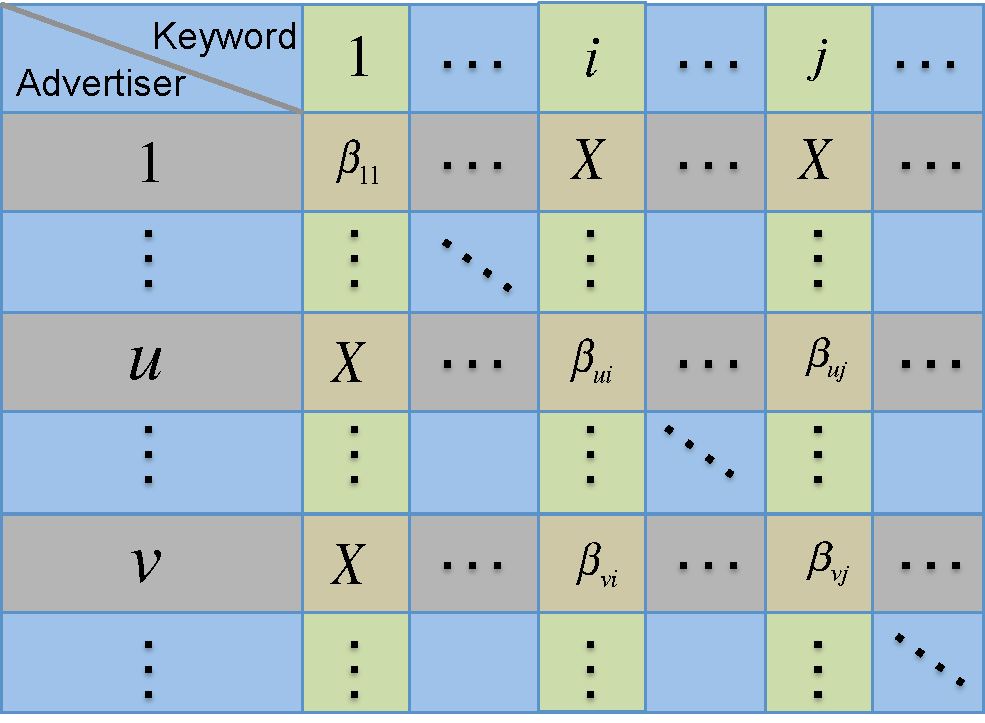
\includegraphics[width=0.35\textwidth]{figures/matrix.pdf}
  \caption{Matrix ??}
  \label{fig:problem-as-matrix}
\end{figure}
We take same settings as other Colleborative Filtering algorithms,
where the input keyword traffic data can be viewed as a matrix, as
shown in Figure~\ref{fig:problem-as-matrix}. Each row represents an
advertisement and each column represents a keyword. If a keyword $i$
is already associated with advertisement $u$, then we have some
observed traffic value $\beta_{ui}$. Otherwise, no value is observed
(noted as $X$). For convenience, we define the notations we will use
through out this paper in Table~\ref{tab:notations}. Specially $u$ and
$v$ will be used for advertisers, while $i$ and $j$ will be used for
keywords.

\begin{table}[!ht]
  \centering
  \begin{tabular}{|l|l|}
    \hline
    Notation & Description \\ \hline
    $N_a$ & total number of advertisements \\ \hline
    $N_k$ & total number of keywords \\ \hline
    $u$ & the $u$th advertisement, $u\in [1,N_a]$\\ \hline
    $i$ & the $i$th keywords, $i\in [1,N_k]$\\ \hline
    $\Lambda$ & missing values in data matrix $M$\\ \hline
    $\Lambda_{(*,i)}$  & missing values in the $i$th column of matrix $M$\\ \hline
    $\Lambda_{(u,*)}$ & missing values in the $u$th row of matrix $M$\\ \hline
    $\Gamma$ & observed (known) values in the matrix $M$\\ \hline
    $\Gamma_{(*,i)}$ & observed values in the $i$th column of matrix $M$\\ \hline
    $\Gamma_{(u,*)}$& observed values in the $u$th row of matrix $M$\\     \hline
    $\beta_{ui}$& observed value for cell ($u$,$i$) of matrix $M$\\ \hline
    $\hat{\beta}_{ui}$& model estimated value for cell ($u$,$i$) of matrix $M$\\ \hline
  \end{tabular}
  \caption{Notations for {\sppan} Model}
\label{tab:notations}
\end{table}

The quality of the model is evaluated by the standard root mean square
error (RMSE), which is
\[
\sqrt{\frac{1}{N_a * N_k}\sum_u \sum_i \left(\beta_{ui}-\hat{\beta}_{ui}\right)^2}
\]
